\section{Durchf\"uhrung}

\begin{wrapfigure}{r}{.5\linewidth}
    \centering
    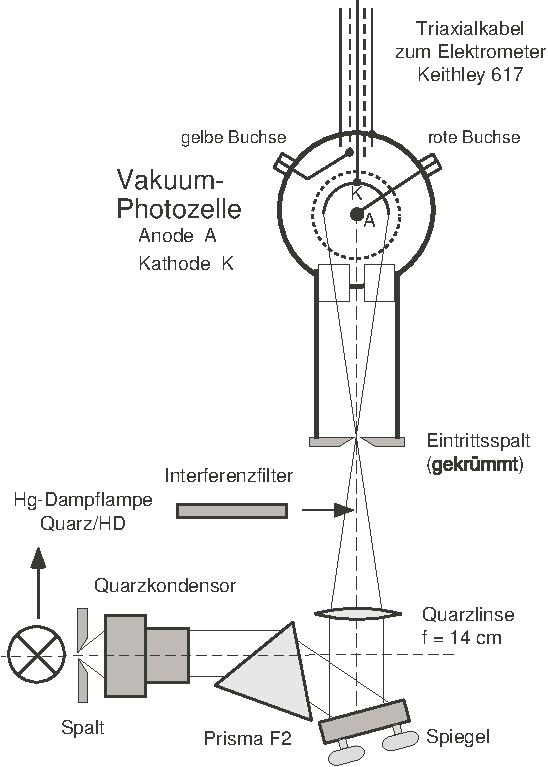
\includegraphics[width=\linewidth]{images/aufbau.pdf}
    \caption{Versuchsaufbau}
\end{wrapfigure}

Das Licht  einer  Hg-Damp-Lampe wird mit Hilfe eines Flint-Prismas F2 spektral
zerlegt und f\"allt \"uber einen Oberfl\"achenspiegel auf  den  Eintrittsspalt
der  Photozelle.  Die Anode ist durch  eine  Blende  abgeschattet.  Wegen  der
unterschiedlichen Lichtwege  im Prisma ist das Spaltbild leicht gekr\"ummt. Es
wird   durch  Verschieben  der  Quarzlinse  scharf  gestellt   und   mit   den
Stellschrauben des Spiegels justiert.  Die  Spaltbreite  ist  so einzustellen,
dass die  Hg-Linien  gelb  und  gr\"un  gerade  deutlich  getrennt  sind.  Vor
Messbeginn muss  man  die  HG-Dampf-Lampe  etwa 10 Min. einbrennen lassen. Zur
Absorption von  UV-Licht  wird  f\"ur alle $\lambda > 400$ \SI{}{\nano\meter} das
Langpassfilter Schott OG 400 zwischen Kondensor und Prisma geschaltet. Bei der
gr\"unen  und  gelben Hg-Linie wird kurzwelligeres  Streulicht  ebenfalls  mit
Hilfe von Kantenfiltern eliminiert.


